\mode<presentation>{

\begin{frame}\frametitle{Unrolling the LSTM in time (the build up - memory states)}
	An alternative visualization of the LSTM cell without delay blocks. We can unroll the network in time to see how the units interact with one another.

	\begin{center}
	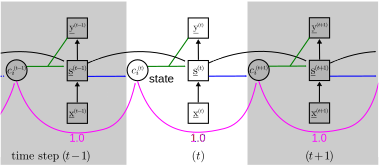
\includegraphics[width=0.9\textwidth]{img/lstm_delay_unroll_memory}
	\captionof*{figure}{Connecting states to hidden \& output units}
	\end{center}
\end{frame}

\begin{frame}\frametitle{Unrolling the LSTM in time (the build up - writing to memory)}
	\begin{center}
	\only<1>{
	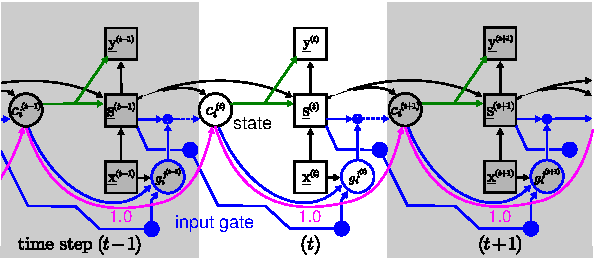
\includegraphics[width=0.9\textwidth]{img/lstm_delay_unroll_write_connect_bubbles}
	\captionof*{figure}{Adding input gates for writing}
	}
	\only<2>{
	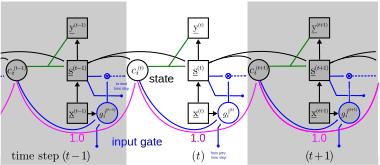
\includegraphics[width=0.9\textwidth]{img/lstm_delay_unroll_write}
	\captionof*{figure}{Adding input gates for writing (keep connections but reduce clutter)}
	}
	\end{center}
\end{frame}
}

\begin{frame}\frametitle{
Unrolling the LSTM in time
(the build up - reading from memory)
}

\mode<article>{
\underline{Unrolling the LSTM in time}:\\

An alternative visualization of the LSTM cell without delay blocks. We can unroll the network in time to see how the units interact with one another.
}

\mode<presentation>{
\placeimage{11.7}{2.2}{img/lstm_delay_indices}{width=33mm}
\vspace{22mm}
}

\begin{figure}[h]
	\centering
	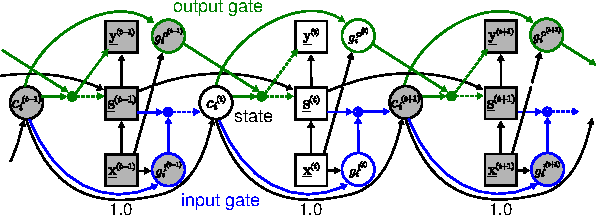
\includegraphics[width=0.9\textwidth]{img/lstm_delay_unroll}
	\mode<article>{
	\caption{Unrolling the LSTM cell with input and output gates in time.}
	}
	\mode<presentation>{
	\captionof*{figure}{Adding output gates for reading}
	}
\end{figure}

\end{frame}
